% Probability Two-Dice Markov Process
%
% File:         probability-two-dice-markov-process.tex
% Author:       Bob Walton (walton@acm.org)
% Date:      	Thu Dec 27 01:19:59 EST 2012
  
\documentclass{minimal}
\usepackage[paperheight=2.4in,paperwidth=6in,
            height=2.4in,hoffset=0.05in,
	    voffset=0.05in,left=0in,width=6in]{geometry}
\usepackage{color}
\usepackage[usenames]{xcolor}
\usepackage{scalefnt}
\usepackage{tikz}
\newcommand{\SMALL}{\scalefont{0.8}}
\usetikzlibrary{arrows}
\begin{document}
\raggedright
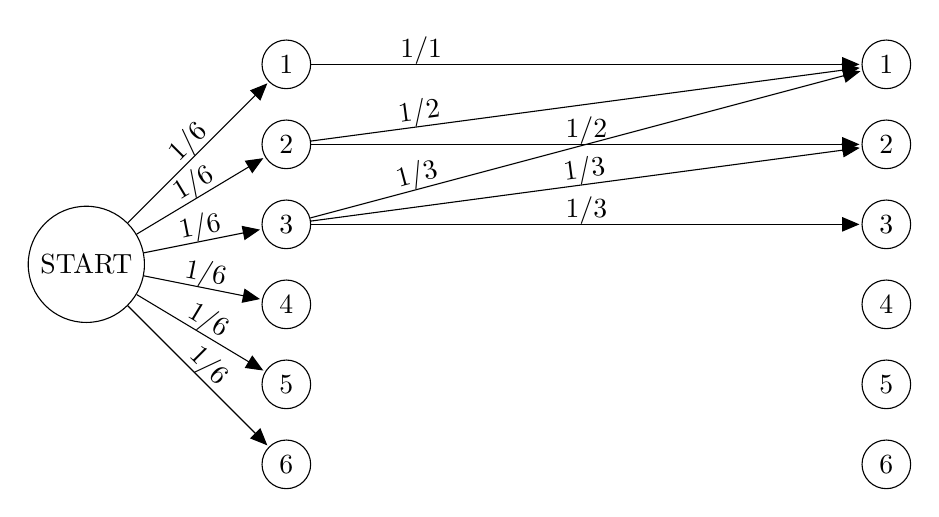
\begin{tikzpicture}[x=1in,y=1in]
\begin{scope}[>=triangle 45,shorten >=0.01in]

    \node[draw,shape=circle] (start) at (0,0) {START};

    \node[draw,shape=circle] (i1)    at (1.0,+1.0) {1};
    \node[draw,shape=circle] (i2)    at (1.0,+0.6) {2};
    \node[draw,shape=circle] (i3)    at (1.0,+0.2) {3};
    \node[draw,shape=circle] (i4)    at (1.0,-0.2) {4};
    \node[draw,shape=circle] (i5)    at (1.0,-0.6) {5};
    \node[draw,shape=circle] (i6)    at (1.0,-1.0) {6};

    \draw[->] (start) -- (i1) node[pos=0.5,sloped,above=-0.05in]{1/6};
    \draw[->] (start) -- (i2) node[pos=0.5,sloped,above=-0.05in]{1/6};
    \draw[->] (start) -- (i3) node[pos=0.5,sloped,above=-0.05in]{1/6};
    \draw[->] (start) -- (i4) node[pos=0.5,sloped,above=-0.05in]{1/6};
    \draw[->] (start) -- (i5) node[pos=0.5,sloped,above=-0.05in]{1/6};
    \draw[->] (start) -- (i6) node[pos=0.5,sloped,above=-0.05in]{1/6};


    \node[draw,shape=circle] (j1)    at (4.0,+1.0) {1};
    \node[draw,shape=circle] (j2)    at (4.0,+0.6) {2};
    \node[draw,shape=circle] (j3)    at (4.0,+0.2) {3};
    \node[draw,shape=circle] (j4)    at (4.0,-0.2) {4};
    \node[draw,shape=circle] (j5)    at (4.0,-0.6) {5};
    \node[draw,shape=circle] (j6)    at (4.0,-1.0) {6};

    \draw[->] (i1) -- (j1) node[pos=0.2,sloped,above=-0.05in]{1/1};

    \draw[->] (i2) -- (j1) node[pos=0.2,sloped,above=-0.05in]{1/2};
    \draw[->] (i2) -- (j2) node[pos=0.5,sloped,above=-0.05in]{1/2};

    \draw[->] (i3) -- (j1) node[pos=0.2,sloped,above=-0.05in]{1/3};
    \draw[->] (i3) -- (j2) node[pos=0.5,sloped,above=-0.05in]{1/3};
    \draw[->] (i3) -- (j3) node[pos=0.5,sloped,above=-0.05in]{1/3};



\end{scope}
\end{tikzpicture}
\end{document}
